% Provenance (never printed): see sources/outline_sources.md (Year 2: oceanic islands; growth,
% flank collapse and erosion of volcanic islands; reefs and atolls; subsidence). Hawaiian
% stages, slides, subsidence and drowned reefs after Clague and Sherrod (2014, USGS PP 1801
% ch. 3) and Denlinger and Morgan (2014, ch. 4); the Nuuanu slide after the ODP Leg 200 report;
% the Enewetak holes after Ladd and Schlanger (1960, USGS PP 260-Y); Kure after the NOAA
% monument pages; the depth--age law from the Book 2 and Book 3 rows. Curves and the invented
% Petrel island from figdata/bachelor-2/islands.py; exercise and problem values in the Book 4
% scratch calculator calc/ch17.py.
\chapter{Pulau Samudra}\label{ch:b2:oceanic-islands}

Pada 1952, di dua pulau \omterm{def:b2:oceanic-islands:reefs}{Atol} Enewetak di Pasifik barat (ketika itu dieja Eniwetok), dua
lubang bor menembus batuan karang sampai lebih dari \qty{1.2}{km}. Di Pulau Parry, mata bor
membawa naik serpihan bor basal segar pada kedalaman 4158 kaki, \qty{1267}{m}, lalu sebuah inti
basal olivin. Di atasnya terletak batu gamping berumur Eosen, penuh karang terumbu dari jenis yang tidak
tumbuh lebih dalam daripada sekitar \qty{46}{m}. Sebuah terumbu karang dulu tumbuh di bahu sebuah gunung api di dekat
muka laut, dan gunung api itu telah tenggelam lebih dari satu kilometer sementara terumbu terus tumbuh di atasnya.
Bab ini mengikuti sebuah \omterm{def:b2:oceanic-islands:stages}{pulau samudra} sepanjang seluruh hidupnya: bagaimana ia tumbuh, bagaimana lerengnya
runtuh ke laut, mengapa ia tenggelam, dan bagaimana sebuah cincin karang dapat bertahan lebih lama daripadanya.
% ledger: ls60:enewetak, ics4:eocene

\begin{recall}
\textbf{Dari volume Tahun 1}: hotspot, plume mantel, jejak hotspot dan progresi umurnya,
rantai Hawaii--Emperor dan Tonjolan Hawaii; hukum kedalaman--umur dasar samudra; terumbu,
bentuk \omterm{def:b2:oceanic-islands:reefs}{terumbu tepi}, \omterm{def:b2:oceanic-islands:reefs}{terumbu penghalang}, dan \omterm{def:b2:oceanic-islands:reefs}{atol} sebagaimana diuraikan Darwin, serta aturan ``mengimbangi atau
tenggelam''; eustasi dan muka laut Maksimum Glasial Terakhir, sekitar \qty{120}{m} lebih rendah daripada
kini. \textbf{Dari volume-volume sekolah}: gunung api perisai; dataran abrasi.
\textbf{Dari \cref{ch:b2:magmatic-series}}: \omterm{def:b2:magmatic-series:series}{seri toleiitik} dan \omterm{def:b2:magmatic-series:series}{seri alkali}.
\end{recall}

\section{Pertumbuhan pulau vulkanik}\label{sec:b2:oceanic-islands:growth}

Kepulauan Hawaii adalah ujung termuda rantai yang diikuti volume Tahun 1 melintasi
Pasifik utara. Pulau-pulau utamanya memuat 19 gunung api perisai yang diketahui: 15 menjulang di atas laut,
3 terbenam, dan satu, yang baru lahir, masih berada di bawah air. Selagi lempeng Pasifik membawanya
ke barat laut, setiap gunung api lahir di atas hotspot, tumbuh, mati selagi hanyut menjauh, dan tenggelam. Hidupnya
cukup teratur untuk dibagi menjadi tahap-tahap.
% ledger: cs14:volcanoes

\begin{definition}[Pulau samudra; tahap-tahap pertumbuhan]\label{def:b2:oceanic-islands:stages}
Yang disebut \emph{pulau samudra}\index{pulau samudra} adalah pulau vulkanik yang menjulang dari dasar
samudra, dibangun di atas litosfer samudra. Sebuah pulau dalam rantai hotspot melalui empat tahap
erupsi: tahap \emph{praperisai} berupa erupsi kecil lava alkali di dasar laut;
\emph{tahap perisai}\index{tahap perisai}, ketika lava toleiitik membangun sebagian besar gunung api
selagi gunung api itu berada di atas hotspot; tahap \emph{pascaperisai} berupa erupsi yang lebih jarang dan lebih alkali,
yang menudungi perisai itu; dan, setelah suatu jeda, tahap \emph{peremajaan} berupa erupsi alkali yang jarang dan
kecil. Erosi dan penenggelaman lalu mengambil alih.
\end{definition}
% ledger: usgs14:hawaii-stages, cs14:rejuvenated

Tahap-tahap itu mengikuti pasokan kalor. Loihi, gunung api terbaru, terletak \qty{54}{km} di selatan
puncak Kilauea; puncaknya masih \qty{975}{m} di bawah laut tetapi sudah \qty{2.5}{km} di atas
dasar laut di sekitarnya, dan lava tertuanya bersifat alkali. Pada \omterm{def:b2:oceanic-islands:stages}{tahap perisai}, gunung api berada di atas
hotspot dan dipasok dengan laju tertinggi. Setiap gunung api Hawaii diperkirakan mengerupsikan 80 sampai
\qty{95}{\percent} volume akhirnya pada tahap ini, sebagian besar dalam 1 sampai \qty{2}{Ma} pertamanya.
Menjelang akhir tahap itu laju erupsi turun dengan faktor sepuluh. Dapur \omterm{def:b2:magma-emplacement:magma}{magma} dangkal, sedalam 1
sampai \qty{7}{km}, tidak dapat lagi dipertahankan, meskipun dapur \omterm{def:b2:magma-emplacement:magma}{magma} yang lebih kecil pada 20 sampai \qty{30}{km}
tetap ada. Lavanya kembali bersifat alkali, karena derajat pelelehan yang lebih rendah menghasilkannya, seperti yang
ditunjukkan \cref{ch:b2:magmatic-series}. Tahap peremajaan datang setelah jeda kurang dari 0.5
sampai \qty{2.0}{Ma}. Tahap itu dapat berupa satu atau dua episode, atau sangat panjang: di Niihau tahap itu berlangsung dari 2.2 sampai
\qty{0.4}{Ma}, dan di Kauai tahap itu telah berlangsung sejak \qty{3.5}{Ma}.
% ledger: cs14:loihi, usgs14:hawaii-stages, cs14:rejuvenated

Volumenya sangat besar. Volume Mauna Loa diperkirakan sekitar \qty{74000}{km^3}. Bila batas dengan Kilauea digambar ulang sehingga Kilauea hanya menyimpan sekitar
\qty{10000}{km^3}, bagian Mauna Loa naik menjadi \qty{95600}{km^3}. Loihi yang muda menyimpan
\qty{1700}{km^3}. Seluruh rantai itu, sejak \qty{81}{Ma}, berjumlah sekitar
\qty{2e6}{km^3}; laju erupsi yang diintegrasikan sepanjang sejarah itu, \qty{0.07}{km^3} per tahun, akan memberikan hampir tiga kali lipatnya. Bebannya cukup berat untuk melengkungkan
lempeng: kerak samudra di bawah pulau-pulau itu tertekan ke bawah sampai sebanyak \qty{5}{km}, di sepanjang
palung yang disebut Parit Hawaii, dan sebuah tonjolan rendah, Lengkungan Hawaii, naik beberapa ratus
kilometer jauhnya. Bagaimana lempeng melengkung di bawah beban dibahas dalam volume Tahun~3. Di sini parit itu
penting karena di sanalah sebagian besar puing pulau-pulau itu berakhir.
% ledger: cs14:volumes, cs14:loihi, cs14:moat

\begin{omfigure}
\centering
\begin{tikzpicture}[x=0.95cm, y=0.95cm, font=\footnotesize]
% schematic, not to scale (vertical exaggeration about 10). Sea level y = 0; sea floor
% y = -1.6 - 0.0625 (16 - x), deepening with the age of the plate to the left.
\fill[omSea!45] (0,0) -- (16,0) -- (16,-1.6) -- (0,-2.6) -- cycle;
\fill[black!18] (0,-2.6) -- (16,-1.6) -- (16,-3.1) -- (0,-3.1) -- cycle;
\draw[black!60] (0,-2.6) -- (16,-1.6);
\draw[omSea!60!black] (0,0) -- (16,0);
\node[anchor=south, font=\scriptsize] at (8.7,0) {muka laut};
% (a) shield stage over the hotspot
\fill[lith basalt, draw=black!70] (12.6,-1.8125) -- (13.9,0.75) -- (14.3,0.9) -- (14.7,0.75) -- (16,-1.6) -- cycle;
% (b) eroded island with a fringing reef (valleys notched in the summit)
\fill[lith basalt, draw=black!70] (9.2,-2.025) -- (10.1,0.15) -- (10.3,0.35) -- (10.45,0.2) -- (10.6,0.45) -- (10.8,0.25) -- (11.0,0.3) -- (11.2,0.1) -- (12.0,-1.85) -- cycle;
\fill[lith reef limestone, draw=black!70] (10.038,0) -- (9.976,-0.15) -- (9.80,0) -- cycle;
\fill[lith reef limestone, draw=black!70] (11.241,0) -- (11.303,-0.15) -- (11.46,0) -- cycle;
% (c) barrier reef around a smaller island, a lagoon between
\fill[lith basalt, draw=black!70] (5.8,-2.2375) -- (7.0,0.2) -- (8.2,-2.0875) -- cycle;
\fill[lith reef limestone, draw=black!70] (6.384,-1.05) -- (6.42,0) -- (6.60,0) -- (6.62,-0.45) -- (6.680,-0.45) -- cycle;
\fill[lith reef limestone, draw=black!70] (7.656,-1.05) -- (7.62,0) -- (7.44,0) -- (7.42,-0.45) -- (7.341,-0.45) -- cycle;
% (d) atoll: volcano bevelled and drowned, reef cap with a lagoon
\fill[lith basalt, draw=black!70] (2.7,-2.43125) -- (3.6,-0.55) -- (4.0,-0.55) -- (4.9,-2.29375) -- cycle;
\fill[lith reef limestone, draw=black!70] (3.4325,-0.9) -- (3.47,0) -- (4.14,0) -- (4.1806,-0.9) -- (4.0,-0.55) -- (3.6,-0.55) -- cycle;
\fill[omSea!45] (3.62,-0.15) rectangle (3.99,0);
% (e) guyot: flat top with a drowned reef cap, beyond the Darwin point
\fill[lith basalt, draw=black!70] (0.2,-2.5875) -- (0.9,-0.95) -- (1.7,-0.95) -- (2.4,-2.475) -- cycle;
\fill[lith reef limestone, draw=black!70] (0.9,-0.95) -- (0.96,-0.75) -- (1.64,-0.75) -- (1.7,-0.95) -- cycle;
% Darwin point
\draw[black!70, dashed] (2.55,0.55) -- (2.55,-2.5);
\node[anchor=south, font=\scriptsize] at (2.55,0.55) {titik Darwin};
% hotspot and plate motion
\draw[omThm, line width=1.4pt, -{Stealth[length=2.5mm]}] (14.3,-3.9) -- (14.3,-3.15);
\node[anchor=west, font=\scriptsize, text=omThm] at (14.4,-3.7) {hotspot};
\draw[black, line width=0.8pt, -{Stealth[length=2.5mm]}] (9.5,-2.85) -- (6.5,-2.85);
\node[anchor=west, font=\scriptsize] at (9.6,-2.85) {gerak lempeng};
\node[anchor=west, font=\scriptsize] at (0.1,-2.9) {litosfer samudra};
% stage labels
\node[align=center, font=\scriptsize] at (14.3,1.45) {(a) tahap perisai};
\node[align=center, font=\scriptsize] at (10.6,1.3) {(b) pulau tererosi,\\ terumbu tepi};
\node[align=center, font=\scriptsize] at (7.0,1.45) {(c) terumbu penghalang};
\node[align=center, font=\scriptsize] at (3.8,1.45) {(d) atol};
\node[align=center, font=\scriptsize] at (1.3,1.45) {(e) guyot};
\draw[black!60, -{Stealth[length=2mm]}] (13.6,-3.7) -- (0,-3.7);
\node[anchor=south, font=\scriptsize, fill=white, inner sep=1pt] at (7,-3.7) {gunung api lebih tua, lempeng lebih tua dan lebih dalam};
\end{tikzpicture}
\par\smallskip{\small Riwayat hidup sebuah \omterm{def:b2:oceanic-islands:stages}{pulau samudra}, dibaca di sepanjang rantai hotspot (skematis, tidak
berskala, skala vertikal sangat dilebih-lebihkan). Lempeng membawa setiap gunung api menjauh dari hotspot
(kanan) dan gunung api itu tenggelam bersamanya, sementara erosi mengikisnya. (a)~Gunung api perisai tumbuh di atas
hotspot. (b)~Setelah padam dan tererosi, gunung api itu dikelilingi \omterm{def:b2:oceanic-islands:reefs}{terumbu tepi}. (c)~Setelah tenggelam lebih jauh, gunung api itu dikelilingi
oleh \omterm{def:b2:oceanic-islands:reefs}{terumbu penghalang} dengan laguna di belakangnya. (d)~Puncaknya telah hilang di bawah laut, dan tudung terumbu dengan
laguna di tengahnya, yaitu \omterm{def:b2:oceanic-islands:reefs}{atol}, tumbuh di atasnya. (e)~Setelah terbawa ke air yang terlalu dingin bagi terumbu untuk
mengimbangi, \omterm{def:b2:oceanic-islands:reefs}{atol} itu tenggelam dan turun sebagai \omterm{def:b2:oceanic-islands:seamount}{guyot} berpuncak datar.}
\end{omfigure}
% ledger: cs14:volcanoes, cs14:erase, cs14:darwin-point, pmnm:geology

\section{Keruntuhan lereng}\label{sec:b2:oceanic-islands:collapse}

Gunung api setinggi beberapa kilometer, yang dibangun dari aliran lava dan reruntuhan yang lepas, berdiri di atas lereng yang
turun ke dalam parit, tidaklah stabil. Pada 1975 gempa bumi Kalapana, bermagnitudo 7.7, menggerakkan
lereng selatan Kilauea sampai \qty{10}{m} ke arah laut dalam sekali gerak dan membangkitkan tsunami. Pada
1868, gerakan lereng yang lain datang bersama gempa bumi bermagnitudo 7.9 dan tsunami yang menewaskan 46
orang. Profil seismik di bawah lereng-lereng itu menunjukkan sebuah reflektor dalam. Reflektor itu dibaca sebagai
\omterm{def:b2:alpine-orogen:decollement}{décollement} di sepanjang puncak kerak samudra lama, tempat seluruh lereng itu meluncur. Biasanya
lereng itu merayap; kadang-kadang lereng itu runtuh.
% ledger: dm14:flank

\begin{definition}[Keruntuhan lereng; longsoran puing; nendatan]\label{def:b2:oceanic-islands:collapse}
Yang disebut \emph{keruntuhan lereng}\index{keruntuhan lereng} adalah runtuhnya sebagian besar lereng
gunung api, yang meluncur menjauh di bawah beratnya sendiri. Bila massa yang bergerak itu pecah dan meluncur
cepat, sebagai aliran blok dan reruntuhan yang dapat menempuh jarak jauh melampaui kaki gunung api, massa itu disebut
\emph{longsoran puing}\index{longsoran puing}. Bila massa itu bergerak lambat, sebagai blok-blok besar yang berotasi
pada sesar-sesar yang berakar di \omterm{def:b2:alpine-orogen:decollement}{décollement} dalam dan tetap berada di dekat gunung api, massa itu disebut \emph{nendatan}.
\end{definition}

Buktinya terletak di bawah laut. Pada akhir 1980-an, pemetaan sonar sapuan samping di perairan sekitar
Kepulauan Hawaii menunjukkan puing yang berserakan di dasar laut dalam, beberapa ratus kilometer dari
pulau-pulau itu, dan nendatan yang terdiri atas blok-blok besar yang tersegmentasi. Tujuh belas longsoran besar dikenali
di sekitar pulau-pulau utama, yang terbentuk dalam \qty{5}{Ma} terakhir. Tujuh puluh kini diketahui di sepanjang
Punggungan Hawaii antara Pulau Hawaii dan Midway, yang terbentuk selama \qty{30}{Ma}. Itu berarti sedikitnya
satu longsoran setiap \qty{300}{ka} di sekitar pulau-pulau utama. Hitungan ini adalah nilai minimum, karena
gunung api yang lebih muda dapat mengubur bekas luka dan puing gunung api yang lebih tua: \omterm{def:b2:eruptive-styles:caldera}{kaldera} puncak dan sebuah zona celah
Niihau hilang, dan tidak ada endapan yang ditemukan untuk keduanya. Longsoran raksasa tampaknya paling mungkin terjadi selagi
gunung api tumbuh paling cepat, dari akhir tahap praperisai sampai awal tahap pascaperisai, tetapi longsoran itu berlanjut
lama sesudahnya.
% ledger: cs14:slides, dm14:flank

Yang terbesar adalah longsoran Nuuanu, yang merobek lereng timur laut gunung api Koolau
di Oahu. Longsoran itu adalah \omterm{def:b2:oceanic-islands:collapse}{longsoran puing} yang tersebar di atas \qty{23000}{km^2}, yang membentang lebih dari
\qty{200}{km} dari pulau itu. Blok-bloknya mencakup Gunung Laut Tuscaloosa, sekitar \qty{30}{km} panjangnya,
\qty{17}{km} lebarnya, dan sedikitnya \qty{2}{km} tingginya. Longsoran itu menyeberangi parit yang dalam dan mendaki
lebih dari \qty{100}{km} ke atas lereng Lengkungan Hawaii. Umurnya diperkirakan 2.1 sampai
\qty{1.8}{Ma}, di dekat akhir hidup Koolau atau sesudahnya, yang lava permukaannya berumur 1.8 sampai
\qty{2.6}{Ma}. Dari berapa keruntuhan longsoran itu tersusun, dan berapa tebalnya jauh dari pulau itu,
masih merupakan pertanyaan terbuka.
% ledger: odp200:nuuanu

\begin{omfigure}
\centering
\begin{tikzpicture}[x=0.95cm, y=0.95cm, font=\footnotesize]
% schematic section from the summit of an island (left) across the moat to the arch (right);
% not to scale. Sea level y = 0; top of the old oceanic crust, bent down under the island.
\fill[omSea!45] (0,0) -- (15,0) -- (15,-2.2) -- (13.5,-2.12) -- (11,-2.05) -- (8.5,-2.35) -- (6.5,-2.75) -- (5.6,-2.82) -- (4.0,-1.4) -- (2.5,0) -- cycle;
\fill[black!18] (0,-3.05) -- (5.6,-2.82) -- (6.5,-2.75) -- (8.5,-2.35) -- (11,-2.05) -- (13.5,-2.12) -- (15,-2.2) -- (15,-3.6) -- (0,-3.6) -- cycle;
\draw[black!70] (0,-3.05) -- (5.6,-2.82) -- (6.5,-2.75) -- (8.5,-2.35) -- (11,-2.05) -- (13.5,-2.12) -- (15,-2.2);
\draw[omSea!60!black] (0,0) -- (15,0);
\node[anchor=south east, font=\scriptsize] at (15,0) {muka laut};
% the volcano: present flank (after collapse) and the lost flank (dashed)
\fill[lith basalt, draw=black!70] (0,1.15) -- (0.8,1.05) -- (1.25,0.95) -- (1.45,0.45) -- (1.75,0.1) -- (2.6,-0.75) -- (3.6,-1.6) -- (4.6,-2.4) -- (5.6,-2.82) -- (0,-3.05) -- cycle;
\draw[black!70, dashed] (1.25,0.95) -- (2.5,0) -- (4.0,-1.4) -- (5.6,-2.82);
\node[font=\scriptsize, align=center, fill=white, inner sep=1pt] at (0.8,-1.6) {gunung api};
\node[font=\scriptsize, anchor=south west, align=left] at (2.0,0.25) {bekas luka\\ lereng yang hilang};
% slump: blocks rotated on listric faults rooted in the decollement
\draw[black, line width=0.7pt] (1.45,0.45) .. controls (1.7,-1.4) and (2.4,-2.6) .. (3.6,-2.95);
\draw[black, line width=0.7pt] (2.6,-0.75) .. controls (2.8,-1.8) and (3.3,-2.6) .. (4.4,-2.9);
\draw[omThm, line width=1.1pt] (0.6,-3.03) -- (5.6,-2.82);
\node[anchor=north, font=\scriptsize, text=omThm] at (2.9,-3.05) {décollement};
% debris avalanche: hummocky sheet across the moat and up the arch, with blocks
\fill[lith conglomerate, draw=black!70] (4.6,-2.4) -- (5.6,-2.62) -- (6.5,-2.6) -- (8.5,-2.22) -- (11,-1.95) -- (12.6,-2.03) -- (11,-2.05) -- (8.5,-2.35) -- (6.5,-2.75) -- (5.6,-2.82) -- cycle;
\fill[lith basalt, draw=black!70] (7.0,-2.62) -- (7.25,-2.25) -- (7.95,-2.22) -- (8.1,-2.43) -- cycle;
\fill[lith basalt, draw=black!70] (9.3,-2.2) -- (9.45,-2.02) -- (9.75,-2.0) -- (9.85,-2.17) -- cycle;
\fill[lith basalt, draw=black!70] (10.6,-2.05) -- (10.7,-1.93) -- (10.9,-1.92) -- (10.95,-2.03) -- cycle;
\draw[black!70] (7.6,-2.2) -- (7.4,-1.3) node[anchor=south, font=\scriptsize, align=center] {blok selebar\\ beberapa km};
\node[anchor=south, font=\scriptsize, align=center] at (10.3,-1.3) {longsoran puing};
\draw[black!70] (10.3,-1.3) -- (10.0,-1.98);
\node[font=\scriptsize] at (6.6,-3.2) {parit};
\node[font=\scriptsize] at (11.6,-2.6) {lengkungan};
\node[anchor=west, font=\scriptsize] at (12.6,-3.3) {kerak samudra};
\draw[black!70] (2.55,-1.55) -- (3.35,-0.6) node[anchor=west, font=\scriptsize, inner sep=1pt] {nendatan};
\draw[black!60, {Stealth[length=2mm]}-{Stealth[length=2mm]}] (5.6,-3.95) -- (12.6,-3.95);
\node[anchor=north, font=\scriptsize] at (9.1,-3.95) {sampai sekitar \qty{200}{km}};
\end{tikzpicture}
\par\smallskip{\small \omterm{def:b2:oceanic-islands:collapse}{Keruntuhan lereng} sebuah \omterm{def:b2:oceanic-islands:stages}{pulau samudra} (skematis, tidak berskala). Di dekat
gunung api, nendatan bergerak lambat sebagai blok-blok yang berotasi pada sesar-sesar yang berakar di \omterm{def:b2:alpine-orogen:decollement}{décollement} di puncak
kerak samudra lama. \omterm{def:b2:oceanic-islands:collapse}{Longsoran puing} terlepas dari lereng, meninggalkan bekas luka, dan meluncur sebagai
lembaran reruntuhan yang membawa blok-blok selebar beberapa kilometer. Longsoran Nuuanu menyeberangi parit
dan mendaki ke atas lengkungan, lebih dari \qty{200}{km} dari Oahu.}
\end{omfigure}
% ledger: dm14:flank, odp200:nuuanu, cs14:moat

Longsoran yang jatuh ke laut menyingkirkan air. Di Lanai dan Molokai, breksi kacau
dari karang dan lava menjulang sampai \qty{155}{m} di atas muka laut dan telah dibaca sebagai endapan
gelombang raksasa yang dibangkitkan oleh keruntuhan. Tafsiran itu diperdebatkan. Sebagian penulis menjelaskan endapan itu dengan
pengangkatan pulau-pulau itu, meskipun terumbu tenggelam di selatan Lanai tidak menunjukkan tanda pengangkatan seperti itu.
Kira-kira sepertiga longsoran raksasa Hawaii adalah \omterm{def:b2:oceanic-islands:collapse}{longsoran puing} yang mampu membangkitkan gelombang besar. Bagaimana
bahaya seperti itu, yang jarang tetapi sangat besar, ditimbang adalah pertanyaan untuk \cref{ch:b2:geological-hazards}.
% ledger: cs14:megatsunami

\section{Mengapa pulau samudra tenggelam}\label{sec:b2:oceanic-islands:subsidence}

Dua proses membuat \omterm{def:b2:oceanic-islands:stages}{pulau samudra} tenggelam, dan keduanya bertumpang tindih. Yang pertama adalah pembebanan: selagi gunung api
tumbuh, beratnya menekan lempeng ke bawah. Fase cepat ini berlangsung mungkin sejuta tahun dan
menenggelamkan garis pantai dan terumbu lebih dari satu kilometer. Di lepas pantai barat laut Pulau
Hawaii, terumbu tenggelam yang berumur diketahui memberikan laju penenggelaman \qty{2.6}{m} per seribu tahun. Gunung api
kecil dapat tenggelam seluruhnya dalam fase ini: Mahukona, di samping Pulau Hawaii, sempat menjadi
pulau dan kini puncaknya berada sekitar \qty{1100}{m} di bawah air. Proses kedua adalah
pendinginan lempeng, yang berlangsung selama seratus juta tahun, dan yang dinyatakan dalam angka oleh subbab ini.
% ledger: cs14:subsidence, cs14:mahukona

Volume Tahun 1 mengukur bagaimana dasar samudra mendalam seiring umurnya $t$ (dalam \unit{Ma}). Dalam
bentuk yang dipakai dalam bab ini:
\[
d(t) = \qty{2500}{m} + C\sqrt{t}, \qquad C = \qty{350}{m.Ma^{-1/2}}, \qquad 0 \le t \le 70,
\]
dan, untuk lempeng yang lebih tua daripada sekitar \qty{20}{Ma},
\[
d(t) = \qty{6400}{m} - \qty{3200}{m}\; e^{-t/62.8}.
\]
Kedua bentuk itu sesuai dalam selisih sekitar \qty{20}{m} antara 20 dan \qty{50}{Ma}, dan berpotongan pada
\qty{26}{Ma}.
% ledger: ps77:depth-age (Book 2), parsons:plate-model (Book 3)
% values (islands.py): t_switch 26.27, d_switch 4293.8; root - exp: 20 Myr -7.6, 50 Myr +18.3

\begin{proposition}[Penenggelaman termal sebuah pulau]\label{prop:b2:oceanic-islands:sinking}
Sebuah pulau yang dibangun di atas lempeng berumur $t_1$, terbawa bersama lempeng, membebaninya dengan berat yang
tidak lagi berubah dan tidak mengubah pendinginan lempeng di bawahnya, tenggelam sebesar
\[
S = d(t_2) - d(t_1)
\]
pada saat lempeng mencapai umur $t_2$, dengan laju $\dot S = d'(t)$. Dengan hukum akar,
\[
S = C\left(\sqrt{t_2} - \sqrt{t_1}\right), \qquad \dot S = \frac{C}{2\sqrt t},
\]
dan, dengan hukum eksponensial, $\dot S = (\qty{3200}{m}/\qty{62.8}{Ma})\,e^{-t/62.8}$. Dalam
selang yang sama, lempeng muda membawa pulau-pulaunya turun lebih jauh daripada lempeng tua.
\end{proposition}

\begin{proof}
Bandingkan dua kolom lempeng yang berumur sama, satu di bawah pulau dan satu di bawah samudra
terbuka yang jauh. Keduanya mendingin dengan cara yang sama, karena pulau tidak mengubah pendinginan lempeng. Jadi keduanya menyusut dengan besaran yang sama, dan puncak masing-masing turun dengan besaran
yang sama. Berat pulau itu sendiri sudah setimbang dan tidak lagi berubah, sehingga tidak menambahkan apa-apa
lagi. Kolom samudra terbuka turun sebesar $d(t_2) - d(t_1)$; demikian pula pulau itu. Penurunan terhadap waktu
memberikan lajunya. Untuk klaim terakhir: dalam selang tetap $\Delta$, $C(\sqrt{t_1 + \Delta} -
\sqrt{t_1})$ berkurang seiring bertambahnya $t_1$, karena turunannya, $\frac C2\bigl(1/\sqrt{t_1 + \Delta}
- 1/\sqrt{t_1}\bigr)$, bernilai negatif.
\end{proof}

Proposisi itu sengaja mengabaikan dua hal. Tonjolan hotspot mengangkat lempeng selagi lempeng
melewatinya dan menurunkannya lagi selagi lempeng bergerak menjauh, yang menambah penenggelaman pulau-pulau termuda
(volume Tahun 1 mengukur tonjolan itu). Dan beban berubah selagi gunung api tumbuh, yang merupakan
fase cepat di atas. Setelah keduanya selesai, pulau itu mengikuti dasar samudra.

Lajunya kecil. Pada lempeng berumur \qty{4}{Ma}, hukum akar memberikan \qty{87.5}{m} per juta
tahun, kurang dari sepersepuluh milimeter per tahun. Pada lempeng berumur \qty{100}{Ma}, hukum eksponensial
memberikan \qty{10.4}{m} per juta tahun, atau \qty{0.01}{m} per seribu tahun. Itulah laju yang
terukur di sepanjang sebagian besar Punggungan Hawaii dan Gunung-Gunung Laut Emperor. Fase pembebanan, pada
\qty{2.6}{m} per seribu tahun, sekitar 250 kali lebih cepat.
% ledger: cs14:subsidence; values (islands.py): rate_100 10.37, age_rate10 102.3

\begin{omfigure}
\centering
% figdata/bachelor-2/islands.py part sink
\begin{tikzpicture}
\begin{axis}[width=0.8\linewidth, height=6.2cm, y dir=reverse, xmin=0, xmax=100, ymin=0,
  ymax=3000, xlabel={waktu sejak pulau dibangun (\unit{Ma})},
  ylabel={penenggelaman termal (\unit{m})}, tick label style={font=\scriptsize},
  label style={font=\small}, xtick pos=bottom, ytick pos=left]
\addplot[omThm, line width=1pt] table[x=dt_Myr, y=t2] {figdata/out/bachelor-2-islands-sink.dat};
\addplot[orange!80!black, line width=1pt] table[x=dt_Myr, y=t10] {figdata/out/bachelor-2-islands-sink.dat};
\addplot[blue!70!black, line width=1pt] table[x=dt_Myr, y=t30] {figdata/out/bachelor-2-islands-sink.dat};
\addplot[black!45, line width=1pt] table[x=dt_Myr, y=t60] {figdata/out/bachelor-2-islands-sink.dat};
\node[font=\scriptsize, anchor=south east, inner sep=1pt] at (axis cs:99,2470) {lempeng berumur \qty{2}{Ma}};
\node[font=\scriptsize, anchor=south east, inner sep=1pt] at (axis cs:99,2140) {\qty{10}{Ma}};
\node[font=\scriptsize, anchor=south east, inner sep=1pt] at (axis cs:99,1380) {\qty{30}{Ma}};
\node[font=\scriptsize, anchor=south east, inner sep=1pt] at (axis cs:99,710) {\qty{60}{Ma}};
\draw[black!50, dashed] (axis cs:0,1267) -- (axis cs:58,1267);
\node[font=\scriptsize, anchor=north west, inner sep=1pt] at (axis cs:1,1300) {Enewetak, \qty{1267}{m}};
\end{axis}
\end{tikzpicture}
\par\smallskip{\small Penenggelaman termal sebuah pulau yang terbawa oleh lempengnya, dari hukum kedalaman--umur,
untuk pulau yang dibangun di atas lempeng berumur 2, 10, 30, dan \qty{60}{Ma} (hukum akar sampai umur lempeng
\qty{26}{Ma}, hukum eksponensial sesudahnya, tempat keduanya bertemu). Makin muda lempengnya, makin cepat
dan makin jauh pulau itu tenggelam. Garis putus-putus menandai kedalaman basal di bawah Enewetak, yaitu
tebal batuan terumbu yang harus diberi ruang oleh penenggelaman.}
\end{omfigure}
% ledger: ps77:depth-age (Book 2), parsons:plate-model (Book 3), ls60:enewetak

\section{Terumbu, atol, dan guyot}\label{sec:b2:oceanic-islands:reefs}

Volume Tahun 1 menguraikan tiga bentuk terumbu sebagaimana dijelaskan Darwin, dari terumbu yang mengelilingi
pulau sampai cincin karang di sekeliling laguna, dan berakhir pada sebuah pertanyaan: mengapa pulau-pulau itu tenggelam,
dan seberapa jauh? Subbab sebelumnya telah menjawabnya. Bentuk-bentuk itu kini dapat didefinisikan menurut keadaan
pulau di bawahnya.

\begin{definition}[Terumbu tepi; terumbu penghalang; atol]\label{def:b2:oceanic-islands:reefs}
Yang disebut \emph{terumbu tepi}\index{terumbu tepi} adalah terumbu yang menempel pada pantai sebuah pulau, tanpa
laguna, atau hanya dengan saluran yang sempit dan dangkal, di antara keduanya. Yang disebut \emph{terumbu penghalang}\index{terumbu penghalang}
adalah terumbu yang terpisah dari pantai oleh laguna, di lereng pulau yang telah tenggelam sementara
terumbu itu tumbuh ke atas. Yang disebut \emph{atol}\index{atol} adalah cincin terumbu, dengan pulau-pulau rendah dari puing terumbu,
di sekeliling laguna tanpa batuan vulkanik di atas muka laut: gunung apinya terletak seluruhnya di bawah terumbu.
\end{definition}

\begin{definition}[Gunung laut; guyot]\label{def:b2:oceanic-islands:seamount}
Yang disebut \emph{gunung laut}\index{gunung laut} adalah gunung api di dasar samudra yang puncaknya terletak di bawah muka
laut, entah karena tidak pernah mencapai permukaan atau karena telah tenggelam. Yang disebut
\emph{guyot}\index{guyot} adalah gunung laut berpuncak datar, yang terpangkas oleh gelombang atau ditudungi terumbu ketika
berada di muka laut, lalu tenggelam.
\end{definition}

Jika sebuah terumbu mempertahankan puncaknya di muka laut sementara gunung api tenggelam di bawahnya, batuan terumbu menumpuk secepat
pulau itu turun. Tebal tudungnya lalu merekam penenggelaman itu.

\begin{proposition}[Tebal tudung terumbu]\label{prop:b2:oceanic-islands:cap}
Misalkan batuan vulkanik terakhir sebuah pulau turun di bawah muka laut ketika lempengnya berumur $t_1$, dan misalkan sebuah
terumbu mempertahankan puncaknya di muka laut sejak saat itu, sampai lempeng berumur $t_2$. Jika muka laut telah naik
sebesar $\Delta\eta$ di antara kedua waktu itu (relatif terhadap pusat Bumi), maka tebal tudung terumbu
di atas gunung api itu adalah
\[
H = d(t_2) - d(t_1) + \Delta\eta = C\left(\sqrt{t_2} - \sqrt{t_1}\right) + \Delta\eta
\]
dengan bentuk kedua memakai hukum akar. Tebal itu tidak bergantung pada laju pertumbuhan terumbu,
asalkan laju itu tidak pernah lebih kecil daripada laju naik relatif muka laut.
\end{proposition}

\begin{proof}
Pada $t_1$ puncak gunung api berada di muka laut; pada $t_2$ puncak itu terletak $S = d(t_2) - d(t_1)$ lebih rendah menurut
\cref{prop:b2:oceanic-islands:sinking}, sementara permukaan laut telah naik sebesar $\Delta\eta$. Puncak
terumbu berada di permukaan laut pada kedua waktu itu, dan dasarnya adalah puncak gunung api. Jadi
tebalnya adalah jarak di antara keduanya, $S + \Delta\eta$. Terumbu yang mampu mengimbangi berhenti di
permukaan, sehingga terumbu yang lebih cepat tidak membangun tudung yang lebih tebal; terumbu yang tidak mampu mengimbangi tertinggal
dan tenggelam, yang merupakan aturan yang diingat kembali dari volume Tahun 1.
\end{proof}

Enewetak membenarkan hal ini. Menurut hukum akar, tudung setebal \qty{1267}{m} memerlukan $\sqrt{t_2} - \sqrt{t_1} =
1267/350 = 3.62$: misalnya, gunung api yang terpangkas sampai muka laut di atas lempeng berumur \qty{10}{Ma} dan
terbawa sampai lempeng berumur \qty{46}{Ma}. Itu \qty{36}{Ma}, orde waktu yang
memisahkan dasar Eosen batu gamping itu dari masa kini. Lubang-lubang bor itu juga menunjukkan apa yang
diabaikan proposisi itu. Zona-zona terlindi, tempat aragonit karang telah terlarut atau
terekristalisasi, merekam masa-masa ketika puncak \omterm{def:b2:oceanic-islands:reefs}{atol} berada di atas laut dan hujan jatuh di atasnya.
Muka laut turun dan naik bersama zaman-zaman es, dan tudung itu telah tersingkap dan tenggelam lagi berkali-kali
dalam perjalanannya ke bawah.
% ledger: ls60:enewetak, ics4:eocene; calc/ch17.py: (3.162 + 3.620)^2 = 46.0

\begin{history}[Mengebor menembus atol, 1896--1952]
Teori Darwin membuat ramalan yang hanya dapat diperiksa dengan bor: di bawah \omterm{def:b2:oceanic-islands:reefs}{atol} seharusnya
ada tumpukan tebal batuan terumbu perairan dangkal, yang bertumpu di atas batuan vulkanik. Lubang dalam pertama
di sebuah \omterm{def:b2:oceanic-islands:reefs}{atol} Pasifik dibor di Funafuti dari 1896 sampai 1898 dan berhenti pada 1114 kaki,
\qty{340}{m}, tanpa mencapai gunung apinya. Sebuah lubang di Kita-daito-jima, di selatan Jepang dan di timur Okinawa,
mencapai 1416 kaki pada 1936, dan sebuah lubang di Bikini 2556 kaki pada 1947, dan keduanya tidak mencapainya. Lubang-lubang di Enewetak, pada
1951 dan 1952, adalah yang pertama mencapai fondasi sebuah \omterm{def:b2:oceanic-islands:reefs}{atol}. Di Elugelab, batuan dasar yang keras
ditemui pada 4610 kaki; di Pulau Parry, basal pada 4158 kaki, 450 kaki lebih tinggi, \num{22}~mil
jauhnya. Para pengebor telah menemukan gunung api basal yang menjulang dua mil di atas dasar samudra, yang ditudungi
batu gamping terumbu sejak Eosen. Elugelab dihancurkan dalam uji coba sebuah perangkat termonuklir
tak lama setelah pengeboran berakhir.
\end{history}
% ledger: ls60:holes, ls60:enewetak

\begin{omfigure}
\centering
% figdata/bachelor-2/islands.py part holes
\begin{tikzpicture}
\begin{axis}[width=0.8\linewidth, height=6.0cm, ybar, bar width=16pt, y dir=reverse, ymin=0,
  ymax=1500, enlarge x limits=0.1, symbolic x coords={Funafuti,Kita-daito-jima,Bikini,Eniwetok-K-1B,Eniwetok-F-1,Eniwetok-E-1},
  xtick=data, xticklabels={{Funafuti\\1898},{Kita-daito-jima\\1936},{Bikini\\1947},{Enewetak\\K-1B, 1951},{Enewetak\\F-1, 1952},{Enewetak\\E-1, 1952}},
  xticklabel style={align=center, font=\scriptsize}, ylabel={kedalaman (\unit{m})},
  tick label style={font=\scriptsize}, label style={font=\small}, xtick pos=bottom, ytick pos=left]
\addplot[fill=omLithLime, draw=black!70] table[x=name, y=td_m] {figdata/out/bachelor-2-islands-holes.dat};
\addplot[only marks, mark=-, mark size=9pt, line width=2.2pt, black, unbounded coords=discard, xshift=0pt]
  table[x=name, y=basalt_m] {figdata/out/bachelor-2-islands-holes.dat};
\end{axis}
\end{tikzpicture}
\par\smallskip{\small Lubang-lubang dalam yang dibor di \omterm{def:b2:oceanic-islands:reefs}{atol-atol} Pasifik, dengan tahun selesainya masing-masing:
kedalaman totalnya (batang) dan, di Enewetak, kedalaman batuan dasar basal (tanda hitam)
(\qty{1405}{m} di bawah Elugelab, F-1; \qty{1267}{m} di bawah Pulau Parry, E-1). Kedalaman dikonversi
dari satuan kaki dalam laporan pengeboran.}
\end{omfigure}
% ledger: ls60:holes, ls60:enewetak; values (islands.py): td and basalt in m

\begin{inthefield}[Mengebor sebuah atol]
Di Enewetak para ahli geologi menempatkan lubang-lubang dalam di dekat pantai laguna, tempat mereka mengharapkan
lebih sedikit gua daripada di dekat tepi terumbu yang menghadap laut. Sebagian besar lubang dibor lurus, dengan batuan digerus menjadi
serpihan bor yang dibawa naik oleh fluida pengeboran. Serpihan itu datang terlambat, sehingga tim memperkirakan
keterlambatan ini untuk mengetahui dari kedalaman mana setiap sampel berasal. Pada kedalaman-kedalaman terpilih, tabung inti mengambil
silinder batuan yang utuh. Setelah pengeboran selesai, lubang-lubang itu dipakai sebagai instrumen. Di satu lubang, yang diselubungi
rapat sampai \qty{600}{m}, muka air masih naik dan turun mengikuti pasang samudra, serempak dan
dengan besaran yang sama: batu gamping tudung itu berpori dan penuh gua di seluruh bagiannya. Lubang-lubang lain
mengukur suhu di dalam lubang selagi suhu itu kembali ke kesetimbangan.
\end{inthefield}
% ledger: ls60:methods, ls60:casing (F-1 cased to 1,973 ft = 601 m)

Terumbu tidak harus tenggelam karena pulaunya tenggelam. Karang dan alga koralin membangun beberapa
milimeter per tahun: dalam satu studi modern, terumbu yang didominasi karang bercabang tumbuh \qty{4.2}{mm} per
tahun. Lempeng
yang mendingin mengambil paling banyak sepersepuluh milimeter per tahun. Penenggelaman termal saja tidak akan pernah
melampaui terumbu yang sehat. Terumbu tenggelam ketika sesuatu yang lain berubah: lempeng membawanya ke air
yang terlalu dingin untuk pertumbuhan cepat; muka laut naik lebih cepat daripada yang dapat diikutinya; atau keduanya terjadi sekaligus.
% ledger: perry:chagos (Book 3), cs14:darwin-point

\begin{omfigure}
\centering
% figdata/bachelor-2/islands.py part rates; horizontal lines from the ledger rows
\begin{tikzpicture}
\begin{semilogyaxis}[width=0.8\linewidth, height=6.4cm, xmin=0, xmax=150, ymin=0.005, ymax=100,
  xlabel={umur lempeng (\unit{Ma})}, ylabel={laju (\unit{mm.yr^{-1}})},
  tick label style={font=\scriptsize}, label style={font=\small}, xtick pos=bottom, ytick pos=left]
\addplot[omThm, line width=1.1pt] table[x=t_Myr, y=thermal_mm_yr] {figdata/out/bachelor-2-islands-rates.dat};
\draw[omThm, densely dotted, line width=0.9pt] (axis cs:75,0.01) -- (axis cs:150,0.01);
\node[font=\scriptsize, anchor=south west, inner sep=1pt, text=omThm] at (axis cs:22,0.042) {penenggelaman termal lempeng};
\node[font=\scriptsize, anchor=south west, inner sep=1pt, text=omThm] at (axis cs:96,0.0108) {terukur, Punggungan Hawaii};
\draw[black!70, line width=0.9pt] (axis cs:0,2.6) -- (axis cs:150,2.6);
\node[font=\scriptsize, anchor=north west, inner sep=1pt] at (axis cs:2,2.6) {pembebanan, di lepas Pulau Hawaii};
\draw[green!50!black, line width=0.9pt] (axis cs:0,4.2) -- (axis cs:150,4.2);
\node[font=\scriptsize, anchor=south west, inner sep=1pt, text=green!40!black] at (axis cs:2,4.2) {pertumbuhan terumbu yang produktif};
\draw[blue!70!black, line width=0.9pt] (axis cs:0,12) -- (axis cs:150,12);
\node[font=\scriptsize, anchor=south west, inner sep=1pt, text=blue!70!black] at (axis cs:2,12) {kenaikan rata-rata muka laut pada deglasiasi terakhir};
\draw[blue!70!black, line width=0.9pt, dashed] (axis cs:0,40) -- (axis cs:150,40);
\node[font=\scriptsize, anchor=south west, inner sep=1pt, text=blue!70!black] at (axis cs:2,40) {Meltwater Pulse 1A, sedikitnya};
\end{semilogyaxis}
\end{tikzpicture}
\par\smallskip{\small Laju-laju yang menentukan apakah terumbu mampu mengimbangi, pada skala logaritmik.
Penenggelaman termal lempeng (dari hukum kedalaman--umur) puluhan sampai ratusan kali lebih lambat daripada pertumbuhan
terumbu; garis bertitik adalah laju yang terukur di sepanjang sebagian besar Punggungan Hawaii. Penenggelaman gunung api yang sedang tumbuh
di bawah bebannya sendiri, dan terutama kenaikan muka laut pada akhir zaman es, mendekati
laju pertumbuhan terumbu atau melampauinya.}
\end{omfigure}
% ledger: cs14:subsidence, perry:chagos (Book 3), lambeck14:lgm (Book 2), ipcc:lgm-sea (Book 2)

\begin{definition}[Titik Darwin]\label{def:b2:oceanic-islands:darwin-point}
Yang disebut \emph{titik Darwin}\index{titik Darwin} suatu rantai hotspot adalah tempat, dan waktu setelah
lahirnya gunung-gunung api, ketika pertumbuhan terumbu ke atas, yang melambat di air yang lebih dingin,
tidak lagi mengimbangi penenggelaman pulau-pulau. \omterm{def:b2:oceanic-islands:reefs}{Atol} yang terbawa melampauinya tenggelam dan menjadi
\omterm{def:b2:oceanic-islands:seamount}{guyot}.
\end{definition}

Di rantai Hawaii, terumbu tenggelam sekitar \qty{33}{Ma} setelah gunung apinya lahir. \omterm{def:b2:oceanic-islands:reefs}{Atol}
Kure, di ujung barat laut kepulauan itu, adalah \omterm{def:b2:oceanic-islands:reefs}{atol} karang paling utara di dunia, dan
terletak di \omterm{def:b2:oceanic-islands:darwin-point}{titik Darwin}. Terumbunya masih tumbuh sedikit lebih cepat daripada tenggelamnya \omterm{def:b2:oceanic-islands:reefs}{atol} itu. Setiap
gunung api di luar Midway dan Kure terbenam, dan sebagian besar adalah \omterm{def:b2:oceanic-islands:seamount}{guyot}. Di Gunung Laut Koko, di
rantai Emperor bagian selatan, karbonat diendapkan dari sekitar 50 sampai \qty{16}{Ma}. Lalu alga koralin
laut dalam yang terakhir tenggelam di bawah batas pertumbuhannya, sekitar \qty{150}{m} di bawah laut. Air yang lebih dingin
saja tidak menenggelamkan terumbu, demikian pula penenggelaman saja. Tenggelamnya terumbu memerlukan penenggelaman,
hanyutnya ke utara ke air yang lebih dingin, dan perubahan iklim yang cepat secara bersama-sama.
% ledger: cs14:darwin-point, pmnm:kure, pmnm:geology

\begin{omfigure}
\centering
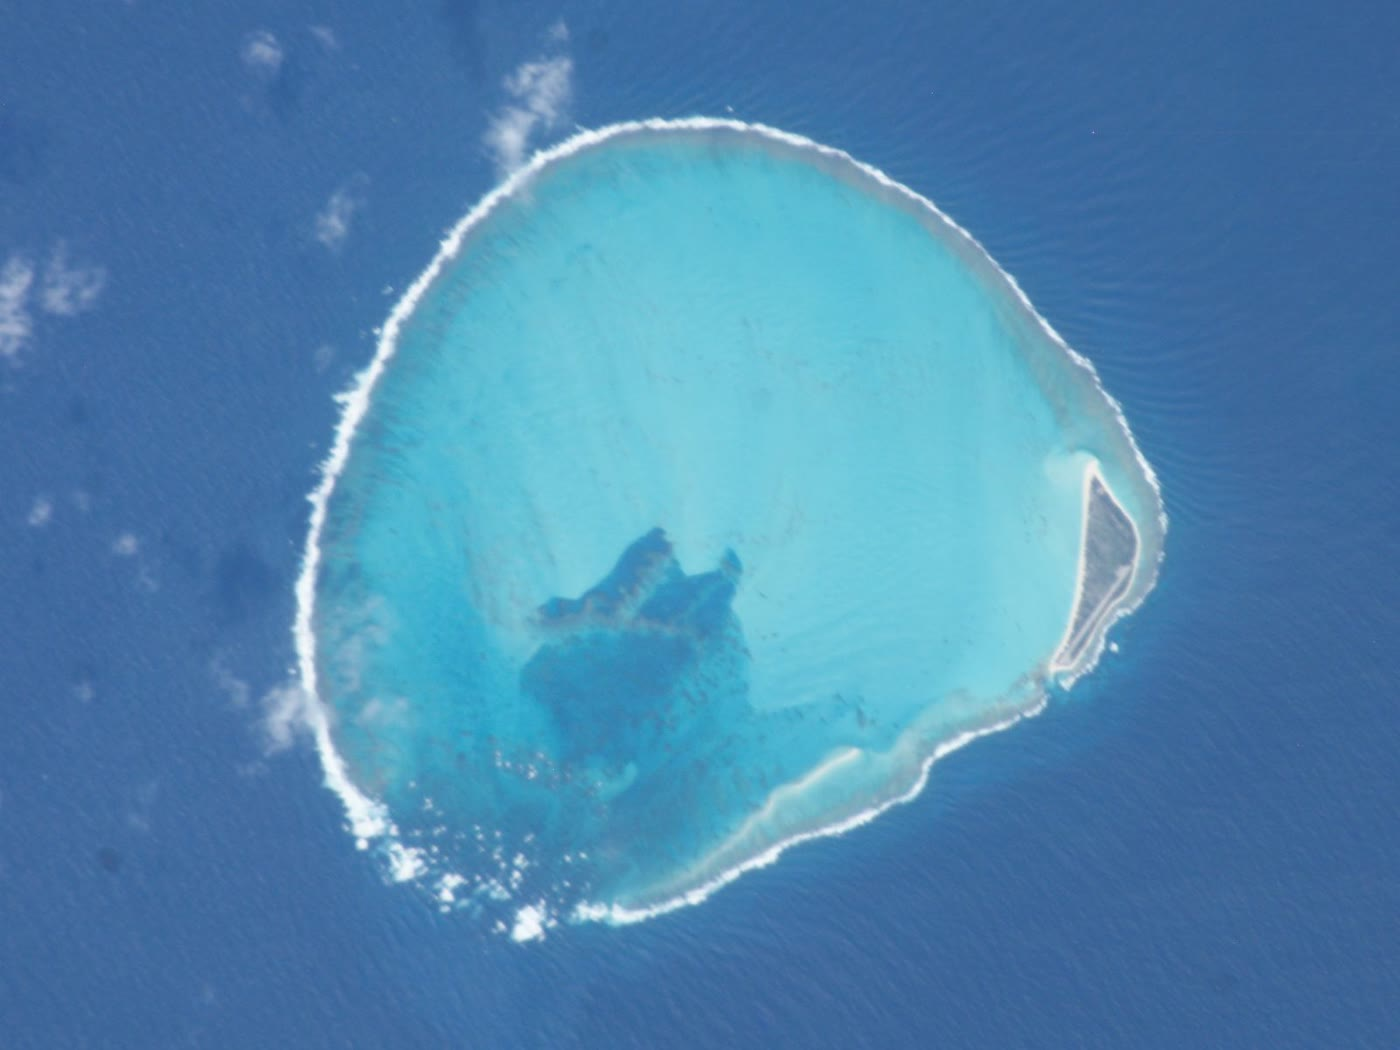
\includegraphics[width=0.52\linewidth]{images/book4/b2-17-kure-atoll.jpg}
\par\smallskip{\small \omterm{def:b2:oceanic-islands:reefs}{Atol} Kure, \omterm{def:b2:oceanic-islands:reefs}{atol} karang paling utara, difoto oleh seorang astronaut dari
Stasiun Antariksa Internasional pada 22 Februari 2004. Cincin terumbunya, yang lebarnya paling banyak sekitar sepuluh kilometer,
melingkupi laguna; satu-satunya pulau permanen, Green Island, terletak di pinggirnya (kanan). Foto: NASA,
domain publik, melalui Wikimedia Commons.}
\end{omfigure}
% ledger: pmnm:kure (6 miles = 9.7 km)

\section{Erosi, muka laut, dan akhir sebuah pulau}\label{sec:b2:oceanic-islands:erosion}

Selagi tenggelam, sebuah pulau juga terkikis. Pulau yang tinggi menangkap angin pasat: di
lereng-lereng gunung api Hawaii yang menghadap angin, di beberapa tempat lebih dari \qty{9}{m} hujan turun dalam setahun.
Sungai-sungai memotong ngarai yang dalam dalam waktu kurang dari sejuta tahun, seperti di Kohala, di Pulau Hawaii.
Sebagian tebing besar yang dulu dianggap hasil erosi saja, seperti tebing laut Molokai
utara, kini dibaca sebagai dinding kepala longsoran raksasa, yang sejak itu mundur oleh erosi. Gelombang menyerang pantai dan
memangkas dataran abrasi di muka laut di sekelilingnya. Erosi dan penenggelaman bersama-sama menghilangkan setiap jejak
batuan vulkanik di atas laut dalam sekitar \qty{15}{Ma}. Gardner Pinnacles, yang berumur sekitar itu, adalah
pulau tertua dalam rantai itu yang batuan vulkaniknya masih menjulang di atas air. Di luarnya ke arah
barat laut hanya ada pulau pasir, \omterm{def:b2:oceanic-islands:reefs}{atol}, dan gunung api yang tenggelam.
% ledger: cs14:erosion, cs14:erase

Muka laut tidak diam selagi semua ini berlangsung. Selama Maksimum Glasial Terakhir muka laut sekitar
\qty{120}{m} lebih rendah daripada kini. Pantai sebuah pulau ketika itu terletak lebih rendah di lerengnya, dan terumbu
yang kini mengelilinginya adalah daratan kering. Ketika es mencair, laut naik rata-rata \qty{12}{m}
setiap seribu tahun selama deglasiasi utama, dari 16.5 sampai \qty{8.2}{ka}. Selama Meltwater
Pulse 1A laut naik sedikitnya \qty{40}{mm} per tahun. Terumbu di atas gunung api yang tenggelam harus mengikuti kedua
kenaikan itu. Di lepas pantai barat laut Pulau Hawaii, sedikitnya enam terumbu tenggelam membentuk
tangga di lereng, yang tertua yang terdalam. Masing-masing tumbuh di pantai, tertinggal selama kenaikan
laut, dan terbawa turun oleh pembebanan pulau muda itu. Begitu sebuah gunung api telah tenggelam lebih
dari sekitar \qty{125}{m}, yaitu rentang muka laut glasial, gunung api itu tidak akan naik kembali ke jangkauan gelombang.
% ledger: usgs:lgm (Book 1), lambeck14:lgm (Book 2), cs14:erase, cs14:subsidence

Lengkungan itu dapat bekerja ke arah sebaliknya. Oahu terletak di atas tonjolan yang terangkat oleh beban pulau-pulau yang lebih muda,
dan telah naik sedikit: terumbu antarglasial terakhir, berumur 133 sampai \qty{115}{ka}, tersingkap di
sekeliling pulau, dan terumbu berumur sekitar \qty{334}{ka} kini berada \qty{21}{m} di atas muka laut. Jadi
akhir sebuah \omterm{def:b2:oceanic-islands:stages}{pulau samudra} tertulis dalam batuan dan terumbunya. Lava membangunnya, longsoran dan
hujan memotongnya, gelombang memangkasnya, lempeng membawanya turun, dan terumbu mempertahankan tempatnya di
permukaan sampai air dingin dan laut yang naik menenggelamkan terumbu itu juga.
% ledger: cs14:arch

\section*{Latihan}\label{sec:b2:oceanic-islands:exercises}

Data untuk latihan, kecuali dinyatakan lain: hukum kedalaman--umur $d = \qty{2500}{m} + C\sqrt t$ dengan
$C = \qty{350}{m.Ma^{-1/2}}$ untuk $0 \le t \le \qty{70}{Ma}$, dan $d = \qty{6400}{m} -
\qty{3200}{m}\,e^{-t/62.8}$ di atas \qty{20}{Ma}; $1~\text{kaki} = \qty{0.3048}{m}$, $1~\text{depa}
= \qty{1.8288}{m}$, $1~\text{mil} = \qty{1.609}{km}$; pertumbuhan terumbu sampai \qty{4.2}{mm.yr^{-1}}.

\begin{exercise}[$\star$]\label{exo:b2:oceanic-islands:1}
Sebutkan tahap setiap gunung api: (a) \omterm{def:b2:oceanic-islands:seamount}{gunung laut} yang puncaknya \qty{975}{m} di bawah laut, yang mengerupsikan
lava alkali; (b) gunung api di atas hotspot, yang mengerupsikan lava toleiitik dengan laju tinggi; (c) gunung api
padam yang aliran terakhirnya, lebih alkali daripada sebagian besar pulau, menudungi perisai; (d)
pulau tempat, setelah diam selama \qty{2}{Ma}, beberapa lubang kepundan alkali yang kecil terbuka; (e) cincin terumbu
di sekeliling laguna tanpa batuan vulkanik yang tampak.
\end{exercise}

\begin{exercise}[$\star$]\label{exo:b2:oceanic-islands:2}
Sebuah gunung api dibangun di atas lempeng berumur \qty{9}{Ma}. (a) Berapa dalam dasar laut di sekitarnya? (b) Seberapa
jauh gunung api itu akan telah tenggelam ketika lempeng berumur \qty{25}{Ma}? (c) Dengan laju berapa gunung api itu tenggelam saat itu?
\end{exercise}

\begin{exercise}[$\star$]\label{exo:b2:oceanic-islands:3}
Tujuh belas longsoran besar terbentuk dalam \qty{5}{Ma} terakhir di sekitar pulau-pulau utama Hawaii, dan
tujuh puluh di sepanjang Punggungan Hawaii dalam \qty{30}{Ma}. (a) Tentukan selang rata-rata antara dua longsoran dalam
masing-masing kasus. (b) Mengapa keduanya hanya merupakan batas atas selang yang sebenarnya?
\end{exercise}

\begin{exercise}[$\star$]\label{exo:b2:oceanic-islands:4}
Di Enewetak, basal ditemui pada 4158 kaki di satu lubang dan batuan dasar yang keras pada 4610 kaki di lubang
yang lain; karang terumbu di dasar batu gamping tidak hidup lebih dalam daripada 150 kaki. (a) Konversikan
ketiga kedalaman itu ke meter. (b) Sedikitnya seberapa jauh puncak gunung api di bawah Pulau Parry telah
tenggelam sejak terumbu pertama tumbuh di atasnya? (c) Dasar batu gamping itu berumur Eosen, jadi sedikitnya
\qty{33.9}{Ma}. Berapa laju rata-rata penenggelaman terbesar yang mungkin?
\end{exercise}

\begin{exercise}[$\star\star$]\label{exo:b2:oceanic-islands:5}
(a) Tentukan laju penenggelaman termal, dalam \unit{m} per \unit{Ma} dan dalam \unit{mm.yr^{-1}}, untuk
pulau-pulau di atas lempeng berumur 4, 25, dan \qty{49}{Ma}. (b) Berapa kali lebih cepat terumbu yang produktif dapat tumbuh
dibandingkan dengan yang tercepat di antaranya? (c) Dan berapa kali lebih cepat fase pembebanan di lepas Pulau
Hawaii, \qty{2.6}{m} per seribu tahun?
\end{exercise}

\begin{exercise}[$\star\star$]\label{exo:b2:oceanic-islands:6}
(a) Dengan hukum eksponensial, tentukan laju penenggelaman pada lempeng berumur \qty{100}{Ma}, dalam \unit{m}
per seribu tahun, dan bandingkan dengan \qty{0.01}{m} per seribu tahun yang terukur di sepanjang
Punggungan Hawaii. (b) Pada umur lempeng berapa lajunya tepat \qty{10}{m.Ma^{-1}}? (c) Periksalah bahwa
kedua hukum memberikan kedalaman yang hampir sama untuk lempeng berumur \qty{25}{Ma}.
\end{exercise}

\begin{exercise}[$\star\star$]\label{exo:b2:oceanic-islands:7}
Terumbu Hawaii tenggelam sekitar \qty{33}{Ma} setelah gunung apinya lahir, dan vulkanisme bergerak
di sepanjang rantai itu dengan laju \qty{8.6}{cm.yr^{-1}}. (a) Seberapa jauh dari hotspot sebuah pulau terletak ketika
terumbunya tenggelam? (b) Midway adalah \omterm{def:b2:oceanic-islands:reefs}{atol} berumur \qty{27.7}{Ma}: apakah konsisten bahwa \omterm{def:b2:oceanic-islands:reefs}{atol} itu masih memiliki
terumbu yang hidup? (c) Kure terletak 55 mil di luar Midway. Perkirakan umurnya, dan katakan apakah \omterm{def:b2:oceanic-islands:reefs}{atol} itu dekat
dengan \omterm{def:b2:oceanic-islands:darwin-point}{titik Darwin}.
\end{exercise}

\begin{exercise}[$\star\star$]\label{exo:b2:oceanic-islands:8}
Dalam \omterm{def:b2:oceanic-islands:collapse}{longsoran puing} Nuuanu, Gunung Laut Tuscaloosa adalah blok sepanjang sekitar \qty{30}{km},
selebar \qty{17}{km}, dan setinggi sedikitnya \qty{2}{km}. (a) Berapa volume yang akan dimuat sebuah kotak berukuran
seperti itu? Dan sebuah limas dengan alas yang sama dan tinggi yang sama? (b) Bandingkan dengan volume
Kilauea, \qty{10000}{km^3}. (c) Longsoran itu menutupi \qty{23000}{km^2}. Jika rata-rata tebalnya
\qty{100}{m} (sebuah asumsi: tebalnya jauh dari Oahu kurang diketahui), berapa
volumenya?
\end{exercise}

\begin{exercise}[$\star\star$]\label{exo:b2:oceanic-islands:9}
Di lepas Pulau Hawaii lereng tenggelam sebesar \qty{2.6}{m} per seribu tahun di bawah beban
gunung api. (a) Berapa lama waktu yang diperlukan untuk menenggelamkan garis pantai sebesar \qty{1}{km}? (b) Sebuah terumbu yang tumbuh dengan laju
\qty{4.2}{mm.yr^{-1}} terletak di lereng ini. Apakah terumbu itu mampu mengimbangi bila muka laut tetap? (c) Selama
deglasiasi utama, dari 16.5 sampai \qty{8.2}{ka}, laut naik rata-rata \qty{12}{mm.yr^{-1}}. Berapa
dalam puncak terumbu di akhir, jika terumbu itu bermula di permukaan? (d) Hal yang sama, untuk terumbu di atas
gunung api tua yang tidak lagi tenggelam.
\end{exercise}

\begin{exercise}[$\star\star\star$]\label{exo:b2:oceanic-islands:10}
(a) Tunjukkan bahwa, dalam selang tetap $\Delta$, hukum akar membuat sebuah pulau tenggelam makin sedikit makin tua
lempengnya. (b) Hitunglah penenggelaman selama \qty{20}{Ma} untuk pulau yang lahir di punggungan dan untuk pulau yang lahir
di atas lempeng berumur \qty{50}{Ma}. (c) Lempeng di bawah punggungan sangat panas, dan hukum akar memberikan laju
tak berhingga pada $t = 0$. Apakah hal itu menjadi masalah bagi penenggelaman dalam selang yang berhingga? Jelaskan.
\end{exercise}

\begin{exercise}[$\star\star\star$]\label{exo:b2:oceanic-islands:11}
Sebuah \omterm{def:b2:oceanic-islands:reefs}{atol} tenggelam dengan laju \qty{30}{m.Ma^{-1}}, dan muka laut berayun sekitar \qty{120}{m} bersama zaman-zaman
es, dalam siklus sekitar \qty{100}{ka}. (a) Seberapa jauh \omterm{def:b2:oceanic-islands:reefs}{atol} itu tenggelam selama satu siklus? (b) Pada
muka laut rendah glasial, seberapa tinggi puncak \omterm{def:b2:oceanic-islands:reefs}{atol} berada di atas laut? Apa yang terjadi pada
batuan terumbu saat itu? (c) Berapa siklus yang diperlukan agar \omterm{def:b2:oceanic-islands:reefs}{atol} tenggelam sebesar seluruh \qty{120}{m}?
(d) Jelaskan zona-zona terlindi yang ditemukan dalam lubang-lubang Enewetak, dan mengapa
\cref{prop:b2:oceanic-islands:cap} tetap memberikan tebal tudung dalam jangka panjang.
\end{exercise}

\begin{exercise}[$\star\star\star$]\label{exo:b2:oceanic-islands:12}
Sebuah \omterm{def:b2:oceanic-islands:reefs}{atol} tenggelam ketika lempengnya berumur \qty{50}{Ma}: terumbunya tertinggal dan puncaknya berakhir di
batas pertumbuhan alga koralin terdalam, \qty{150}{m} di bawah laut. (a) Dengan hukum
eksponensial, seberapa jauh lagi \omterm{def:b2:oceanic-islands:reefs}{atol} itu tenggelam sebelum lempeng berumur \qty{120}{Ma}? (b) Berapa dalam puncak
\omterm{def:b2:oceanic-islands:seamount}{guyot} itu saat itu? (c) Sebuah \omterm{def:b2:oceanic-islands:seamount}{guyot} di samping Enewetak memiliki puncak pada 700 depa. Konversikan, dan bandingkan.
(d) Sebutkan dua alasan mengapa \omterm{def:b2:oceanic-islands:seamount}{guyot} yang sebenarnya dapat lebih dalam atau lebih dangkal daripada taksiran ini.
\end{exercise}

\begin{problem}[{Soal akhir pekan --- Dari gunung api menjadi atol}]\label{pb:b2:oceanic-islands:1}
Pulau Petrel yang rekaan lahir di atas hotspot pada lempeng berumur \qty{10}{Ma}. Gunung apinya
berupa kerucut dengan jari-jari alas \qty{50}{km}. Ketika pertumbuhannya berakhir, puncaknya menjulang \qty{1000}{m} di atas
muka laut. Batuan vulkanik terakhirnya menghilang di bawah muka laut \qty{12}{Ma} kemudian. Sebuah terumbu lalu
mempertahankan puncaknya di muka laut sampai lempeng berumur \qty{70}{Ma}, ketika \omterm{def:b2:oceanic-islands:reefs}{atol} itu melewati
\omterm{def:b2:oceanic-islands:darwin-point}{titik Darwin}. Gunakan hukum kedalaman--umur dari latihan (hukum akar sampai \qty{70}{Ma}, hukum
eksponensial sesudahnya), pertumbuhan terumbu \qty{4.2}{mm.yr^{-1}}, dan data bab ini.
Muka laut dianggap tetap, kecuali dalam pertanyaan 8 sampai 10. Bulatkan kedalaman sampai meter.

\noindent\textbf{Bagian I --- Pertumbuhan.}
\begin{enumerate}
  \item Berapa dalam dasar laut tempat Petrel lahir?
  \item Berapa tinggi gunung api di atas dasar itu ketika pertumbuhannya berakhir, dengan mengabaikan
        penenggelaman dasar di bawah beban?
  \item Tentukan volume kerucut itu.
  \item Jika \qty{85}{\percent} volumenya dierupsikan selama \omterm{def:b2:oceanic-islands:stages}{tahap perisai} yang berlangsung \qty{1}{Ma}, berapa
        laju rata-rata erupsinya? Bandingkan dengan pasokan Kilauea kini, sekitar
        \qty{0.1}{km^3} per tahun.
  \item Berapa Petrel yang akan membentuk satu Mauna Loa, sebesar \qty{95600}{km^3}?
  \item Lava mana, toleiitik atau alkali, yang membentuk sebagian besar kerucut itu? Lava mana yang menudunginya?
\end{enumerate}

\noindent\textbf{Bagian II --- Pembebanan dan terumbu yang tenggelam.}
\begin{enumerate}[resume]
  \item Selama pertumbuhannya, beban menenggelamkan pulau muda itu sebesar \qty{1}{km} dalam \qty{1}{Ma}. Berapa
        laju rata-ratanya, dan bagaimana perbandingannya dengan \qty{2.6}{m} per seribu tahun yang terukur
        di lepas Pulau Hawaii?
  \item Sebuah terumbu tumbuh di pantai selama fase ini, dengan muka laut tetap. Apakah terumbu itu mampu mengimbangi, dan
        dengan selisih berapa?
  \item Muka laut lalu naik dengan laju \qty{12}{mm.yr^{-1}}. Seberapa banyak terumbu itu tertinggal setiap
        tahun?
  \item Berapa lama sampai puncaknya mencapai \qty{150}{m}, batas pertumbuhan terdalam? Apa yang
        ditinggalkannya di lereng pulau itu?
\end{enumerate}

\noindent\textbf{Bagian III --- Penenggelaman dan erosi.}
\begin{enumerate}[resume]
  \item Seberapa jauh Petrel telah tenggelam pada saat batuan vulkanik terakhirnya menghilang, ketika lempeng
        berumur \qty{22}{Ma}?
  \item Berapa banyak dari \qty{1000}{m} puncak itu yang disingkirkan erosi, dan dengan laju rata-rata berapa?
  \item Dengan laju berapa Petrel tenggelam ketika pertumbuhannya berakhir, dan ketika puncaknya menghilang?
  \item Berapa dalam dasar laut di sekitarnya saat itu?
  \item Bandingkan \qty{12}{Ma} yang diperlukannya dengan \qty{15}{Ma} Kepulauan Hawaii. Berikan satu
        alasan mengapa pulau Hawaii yang tinggi bertahan lebih lama.
  \item Sebutkan dua proses, selain hujan dan sungai, yang menyingkirkan pulau itu di atas muka laut.
  \item Bentuk terumbu mana yang mengelilingi Petrel tak lama sebelum puncaknya menghilang?
\end{enumerate}

\noindent\textbf{Bagian IV --- Atol dan guyot.}
\begin{enumerate}[resume]
  \item Berapa tebal tudung terumbu ketika lempeng berumur \qty{70}{Ma}?
  \item Laju rata-rata pertumbuhan terumbu berapa yang diperlukan untuk itu? Berapa kali lebih kecil laju itu daripada pertumbuhan
        yang dapat dicapai terumbu itu?
  \item Bandingkan tudung itu dengan kedalaman basal di bawah Enewetak.
  \item Berapa dalam dasar laut di sekitar \omterm{def:b2:oceanic-islands:reefs}{atol} ketika \omterm{def:b2:oceanic-islands:reefs}{atol} itu melewati \omterm{def:b2:oceanic-islands:darwin-point}{titik Darwin}?
  \item Dengan hukum eksponensial, seberapa jauh lagi \omterm{def:b2:oceanic-islands:reefs}{atol} yang tenggelam itu turun sebelum lempeng berumur
        \qty{120}{Ma}?
  \item Jika puncak terumbu berhenti pada \qty{150}{m} ketika terumbu itu tenggelam, berapa dalam puncak
        \omterm{def:b2:oceanic-islands:seamount}{guyot} itu saat itu?
  \item Sebagai ringkasan: berapa tebal tudung terumbu \omterm{def:b2:oceanic-islands:reefs}{atol} Petrel?
\end{enumerate}
\end{problem}
